\documentclass[
    oneside,
    11pt,
    a4paper
]{utad_msc}

% Packages
\usepackage[autostyle=true]{csquotes}
\usepackage{lmodern} % Support latin modern fonts
\usepackage[T1]{fontenc} % Support for T1 enconding
\usepackage[spanish,activeacute]{babel} % Set spanish language
\usepackage[autostyle=true]{csquotes}
\usepackage{mathtools} % Add additional tools for math writing 

\graphicspath{ {./images/} }
\setcounter{tocdepth}{4}
\setcounter{secnumdepth}{4}

\student{Anxo Babío Rodríguez}
\tutor{Iván Alduán Íñiguez}
\course{Máster en computación gráfica realidad virtual y la simulación}
\project{Materiales PBR en WebGL 2.0}


\AtBeginDocument{%
  \addtocontents{toc}{\protect\thispagestyle{empty}}
}

\begin{document}
    \begin{titlepage}
    \newgeometry{left=2cm,bottom=2cm, top=3.5cm, right=2cm}
    \begin{figure*}
        
\includegraphics[scale=1]{logo_ucjc}\hfill%
        
\includegraphics[scale=1]{logo_utad}%
        \vspace{1cm}
    \end{figure*}
    \title{
        \large \MakeUppercase{\utadcourse} \\
        \vspace{0.5cm}
        \Huge \MakeUppercase{\utadtitle}
        \vfill
    }
    \author{
        AUTOR: \MakeUppercase{\utadstudent} \\
        TUTOR: \MakeUppercase{\utadtutor}
    }
    \date{}
    \maketitle
\end{titlepage}
    1{
    \autocite{killzone}
    \autocite{unreal}
    \autocite{blackopstalk}
    \autocite{blackops}
    \autocite{theordertalk}
    \autocite{theorder}
    \autocite{frostbitetalk}
    \autocite{frostbite}
    \autocite{disney15talk}
    \autocite{disney15}
    \autocite{uncharted4}
    \autocite{pbmwherearewe}
    \autocite{sheenbrdf}
}
    \pagestyle{empty}

    \tableofcontents

    \begingroup
      \frontmatter
        \chapter{Marco colaborativo}
Seddi es una startup nacida como fruto de la investigacion en tecnologias de simulacion optica y mecanica aplicadas al sector textil.
Propone ofrecer una solucion digital que permita a los disenhadores, patronistas o comerciales trabajar en un entorno colaborativo que
representa con gran fidelidad los elementos constructivos de un prenda de ropa: tejido, costuras, dobladillos, etc.

La caida, el brillo y, en general, la apariencia de una prenda son factores clave para validar o rechazar el producto, estas caracteristicas
dependen de propiedades opticas y mecanicas que las herramientas de disenho actuales no tienen en cuenta, por lo que los profesionales del
sector no satisfacen las necesidades de los profesionales de la industria, que en la mayor parte de los casos mantienen un proceso de
trabajo artesanal en el que el prototipado y construccion de la prenda es un proceso iterativo entre patronista y disenhador y cuyo
resultado depende en gran medida de la experiencia y destreza de estos profesionales.

Para ofrecer su solucion, Seddi cuenta con departamentos de investigacion simulacion y captura tanto mecanica como optica, que desarrollan
nuevos algoritmos y hardware que permitan un mayor grado de fidelidad en el momento de captura de los parametros que conforman la apariencia
de una prenda, tanto como mejorar su representacion digital asi como departamentos de desarrollo de producto, se encargan del proceso de
captura utilizando estas tecnologias propietarias asi como de integrar estos algoritmos en diferentes plataformas que permitan al consumidor
final interactuar sobre los tejidos digitales durante diferentes etapas asociadas a este proceso de produccion con el fin de facilitar,
acelerar y reducir los costes de produccion.

Para conseguir un resultado fidedigno, en Seddi, el proceso comienza creando un clon digital del tejido, la obtencion de parametros opticos y
mecanicos que identifican el tejido y se valida utilizando las tecnologias de simulacion y render de la empresa. 

Todos las herramientas de Seddi se alojan en la nube, lo que garantiza disponibilidad inmediata a los recursos a todo el equipo involucrado en
el proceso de produccion. Estos equipos, con un negocio de la moda cada dia mas globalizado, pueden tratarse de equipos multidisciplinares de
diferentes empresas o paises, por lo que es primordial un flujo de comunicacion constante que minimice los errores y los costes economicos y
medioambientales de los flujos de disenho y prototipado

Gracias a esta estrategia de implementación, el contenido diseñado está disponible de manera inmediata y editable en un escenario global. En la
actualidad, el negocio de la moda está completamente globalizado, y las tareas de diseño y prototipado de muchas marcas se hacen entre equipos
internacionales o mediante subcontratación entre empresas. La  utilización de las soluciones cloud de DESILICO permitirá a los equipos colaborar remotamente sobre un mismo diseño.
En Seddi, el proceso para llegar a construir una prenda, comienza con la digitalizacion de un tejido, que se consigue a partir de muestras que
son analizadas por maquinas de captura desarrolladas en Seddi, para obtener los parametros mecanicos y opticos

    \endgroup

    \clearpage
    \pagestyle{fancy}
    \mainmatter % Begin pagination
      \chapter{Introducci\'on}

En Computer Graphics, la tecnica del shading permite mejorar la percepcion de
los volumenes en 3D. Con el aumento de la capacidad de computacion estas tenicas
han evolucionado mucho en un breve periodo de tiempo.\sidenote{Is this correct?}\sidenote{I'm unsure about also!}

Las primeras aportaciones el campo fueron durante los anhos 70 por parte de Bui
Tuong Phong, Henri Gouroud y Jim Blinn con sus modelos de shading: Phong, Gouroud
y Blinn-Phong. Estos algoritmos permiten, a partir de la posicion de la luz, y la
position de la camara, dar una estimacion de la cantidad de luz emitida por una
superficie.\autocite[1]{DUMMY1}

\begin{figure}[H]
    \setlength{\fboxsep}{0pt}
    \fbox{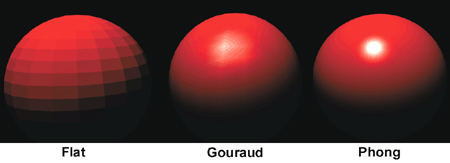
\includegraphics[width=0.99\linewidth]{images/gouroud-phong-flat.jpg}}
    \caption{A boat.}
\end{figure}

\todo[inline]{
    TODO: hablar sobre matriz de perspectiva de
    \href{http://www.cs.uns.edu.ar/cg/clasespdf/p465carlbom.pdf}
    {Ingrid Carlbon}
}

\todo[inline]{
    Siguientes a\~nos: antialising, sombras, multinucleo aparicion GPUs,
    raytracing...
    \href{https://ohiostate.pressbooks.pub/graphicshistory/back-matter/cg-historical-timeline/\#1970}
    {fuente}
}

\todo[inline]{
    Blinn’s law: “as technology advances, rendering time remains constant.” 
    from
    \href{http://www.pbr-book.org/3ed-2018/Introduction/A_Brief_History_of_Physically_Based_Rendering.html}
    {here}
}

\todo[inline]{
    Blinn's law: James Blinn first pointed out, in animation, rendering time remains
    constant, even as computers get faster. An artist gets accustomed to waiting a
    certain number of hours for an image to render, so as hardware improves, instead
    of using it to save time, he employs it to render more complex graphics. from
    \href{https://nevalalee.wordpress.com/2011/08/09/blinns-law-and-the-paradox-of-efficiency/}
    {here}
}

\todo[inline]{
    TODO: Esquema evolucion en el tiempo del shading: phong, blinn-phong
}


      \chapter{Objetivo}
      \chapter{Contexto}
    Seddi es una compañia de computación gráfica especializada en simulación de tejidos para la
    industria de la moda.
    Su objetivo es crear una servicio en la nube en el que las empresa dedicadas a la moda puedan
    digitalizar todo su flujo de trabajo para agilizar el prototipado y reducir costes tanto económicos
    como medioambientales. Para ello se ofrece una plataforma online de trabajo colaborativo con
    herramientas que permiten editar el diseño o las propiedades de una prenda a los diferentes
    perfiles implicados en las fases de producción: diseñadores textiles, diseñadores de moda,
    patronistas, product managers, etc.

\section{Caracteristicas: especial atencion a los tejidos.}
    El motor de render online de Seddi debe ser capaz de mostrar un amplio abanico de materiales,
    pero prestando una especial atenci\'on a los tejidos. Los materiales que pueden ser usados durante
    el proceso de dise\~no de una prenda pueden ir desde cuero, lana, toalla, terciopelo... cada uno
    con unas propiedades opticas y mec\'anicas diferentes y \'unicas que influyen completamente en las
    decisiones de dise\~no del producto.

\section{Author: aplicacion web donde el usuario disenha sus creaciones}
    El proceso empieza con la creación de un digital twin de un hilo, capturando las propiedades
    físicas y mecánicas de las fibras que lo componen y que sirven como entradas a los algoritmos de
    simulación y render. A partir de este hilo los usuarios pueden diseñar un tejido o escoger entre
    una gran cantidad de ellos, en función de la frecuencia o el tipo de entrelazado de los hilos.
    Utilizando estos tejidos se diseñan patrones en plano con las formas de las piezas que conforman
    una prenda y se permite al usuario previsualizar y editar la construcción del modelo en una vista
    3D sobre un maniquí. Una vez completado el ciclo de diseño se generan automáticamente fichas técnicas
    con especificaciones sobre los elementos estéticos o constructivos que facilitan la comunicación
    entre todas las partes implicadas en el proceso de fabricación.
      \chapter{Conceptos previos}

\section{Render}
    El render es un area de la computacion gr\'afica que se encarga de traducir estructuras de datos y funciones a p\'ixeles en la pantalla
    con el objetivo de formar una imagen bidimensional.
    
    La representaci\'on digital de una imagen consiste en un grafo que contiene los elementos de la escena: c\'amara, luces y objetos visibles en
    la escena. Sobre esta escena virtual, se simulan las interacciones de la luz con las superficies para acabar estimando un color para cada
    superficie visible desde el punto de vista de la c\'amara.

    Sus principales aplicaciones se encuentran en industrias como el cine de animaci\'on, los efectos especiales,
    videojuegos, arquitectura, simuladores del \'ambito industrial, visualizaciones de producto o la im\'agen m\'edica.
    Debido a las diferentes necesidades y caracteristicas de cada industria, podemos categorizar a los motores de render
    principalemente en base a dos criterios: su intenci\'on de imitar o no la realidad (motores fotorrealistas y no
    fotorrealistas) y la necesidad o no de interaccion de usuario (motores online y offline).

    En este trabajo, la intencion es el renderizado de telas con el mayor grado de fidelidad posible a la realidad en una
    aplicaci\'on con interaccion de usuario, por lo que nos centraremos en el renderizado online fotorrealista.

    \todo[inline] {
        A\~nadir informaci\~on elementos y grafo de escena. 
        A scene file contains objects in a strictly defined language or data structure; it would contain geometry, viewpoint, texture, lighting, and shading information as a description of the virtual scene.
        The data contained in the scene file is then passed to a rendering program to be processed and output to a digital image or raster graphics image file. 
        If a scene is to look relatively realistic and predictable under virtual lighting, the rendering software should solve the rendering equation
    }

\section{Modelo f\'isico de la luz}
    Para conseguir im\'agenes parecidas a la realidad, el render utiliza algoritmos que simulan el comportamiento f\'isico de la luz.
    El comportamiento de los fotones se describe con el fenomeno cuantico conocido como dualidad onda-part\'icula. El comportamiento
    como particula establece que se mueve en linea recta, rebotando con los objetos del entorno a una velocidad de 300.000 km/s,
    la mas alta conocida y que en el modelo de simulaci\'on se considera infinita. Por otra parte, el comportamiento de de la luz como
    onda, permite trabajar sobre propiedades como frecuencia, amplitud y longitud de onda, que se utilizan para modelar la representaci\'on
    digital del color .
    \todo[inline] {
        Inverse square law. Ley de Lambert. Ley de reflexion. Ley de Snell
    }

\section{Color}
    La interpretaci\'on del color depende de dos cosas, por una parte, las longitudes de onda que inciden sobre una superficie, y como
    esta superficie absorve o refleja esas longitudes de onda y por otra parte, como nuestros receptores reaccionan al espectro visible.
    
    La fotometr\'ia estudia la percepci\'on de la luz por el ojo humano, mientras que la radiometr\'ia se encarga del estudio del fen\'omeno
    f\'isico y es en la que se centra el render para la simulacion f\'isica de la escena tridimensional.
    Para medir la luz se utiliza el espectro, una gr\'afica cartesiana en la que se mide sobre el eje x la longitud de onda y en el eje y,
    su amplitud. El rango de longitudes de onda que se utiliza en render esta limitado a las longitudes de onda visibles por el ojo humano,
    que se conoce como espectro visible. Las ondas de luz pueden sumarse, como se suman las senhales y dar como resultado un nuevo color.
    
    En las aplicaciones de software, la representacion del espectro completo es muy costoso, por lo que se suele trabajar con una
    simplificacion del modelo, la combinacion de espectros base o la descomposicion en funciones base.
    Una de los representaciones mas populares es el modelo RGB, que se corresponde con los tres tipos de conos del ojo humano, los mas
    sensibles al verde, al rojo y al azul.  Es un modelo aditivo, por lo que cada color se obtiene a partir de la suma de estos tres. Aunque
    existen otras representaciones digitales del color, dependiendo de su aplicaci\'on, CMYK, XYZ, etc. el RGB es el mas comun en el mundo de
    la computacion gr\'afica.

\section{Unidades de medida de la luz}
    Cuando hablamos de la cantidad de luz, no es la medicion sobre un foton de luz independiente, si no que se tratan de medidas en relacion
    al tiempo, la direccion o el \'area.

    \subsection{\'Angulo s\'olido}

    \subsection{Flujo}
        La unidad que representa la energia sobre la unidad de tiempo es el flujo, representado por Phi. Es la energía que transportan las ondas
        por unidad de tiempo, se mide en vatios. En los motores de render se utiliza para expresar la cantidad total de energia emitida por un a fuente de luz.
        \begin{equation}
            \Phi_e = \dfrac{d{Q_e}}{dt}
        \end{equation}
        \singlespacing

    \subsection{Intensidad}
        \begin{equation}
            I = \dfrac{d\Phi}{d\omega}
        \end{equation}
        \singlespacing

    \subsection{Irradiancia}
        La irradiancia, es la cantidad de energ\'ia por unidad de tiempo por unidad de superficie, o flujo por superficie. Se representa como
        E, su unidad son los vatios/m2 y se utiliza para medir la cantidad de luz que incide sobre una superficie.
        \begin{equation}
            E = \dfrac{d\Phi}{dA}
        \end{equation}
        Cuando este flujo de radiancia se mide en direcci\'on contraria, de salida, se llama emitancia (M)
        \singlespacing

    \subsection{Radiancia}
        \begin{equation}
            L = \dfrac{d^2\Phi}{dA_{proj}d\omega}
        \end{equation}


\section{Ecuaci\'on de render}
    El prop\'osito de la ecuacion de render es conocer el valor de radiancia que llega a la camara en una direcci\'on
    por cada pixel  de la camara.

    Para saber la radiancia sobre un punto en una direcci\'on, utilizamos la ecuacion de reflectancia, que depende
    de la luz que llega al puntos, el coseno del angulo con el que incide la luz y el BRDF (bidirectional reflectance
    distribution function), que modela el comportamiento de la luz al rebotar sobre la superficie.
    \begin{equation}
        L(x\xrightarrow{}{\vec{v}{\,}})
        = L_i(x\xleftarrow{}{\vec{l}{\,}})
        f(x, \vec{v}{\,}, \vec{l}{\,})
        (\vec{l}{\,}\cdotp{\vec{n}{\,}})
    \end{equation}
    \singlespacing

    Ademas de recibir la luz directamente de una fuente de luz, el punto tambi\'en puede recibir luz rebotada por otras
    partes del entorno:
    \begin{equation}
        L(x\xrightarrow{}{\vec{v}{\,}})
        = L_e(x, \vec{v}{\,}) +
        L_i(x\xleftarrow{}{\vec{l}{\,}})
        f(x, \vec{v}{\,}, \vec{l}{\,})
        (\vec{l}{\,}\cdotp{\vec{n}{\,}})
    \end{equation}
    \singlespacing

    Podr\'iamos sumar todas las fuentes de luz para calcular la radiancia total debido a las fuentes de luz:
    \begin{equation}
        L(x\xrightarrow{}{\vec{v}{\,}})
        = L_e(x, \vec{v}{\,}) +
        \sum{}L_i(x\xleftarrow{}{\vec{l_i}{\,}})
        f(x, \vec{v}{\,}, \vec{l_i}{\,})
        (\vec{l_i}{\,}\cdotp{\vec{n}{\,}})
    \end{equation}
    \singlespacing

    Sin embargo, para tener en cuenta el total de luz incidente, ademas de las fuentes de luz (luz directa), debemos
    de tener en cuenta toda la luz proviniente del entorno en todas direcciones (luz indirecta):
    \begin{equation}
        L(x\xrightarrow{}{\vec{v}{\,}})
        = L_e(x, \vec{v}{\,}) +
        \int_{\Omega}L_i(x'\xrightarrow{}{\vec{l_i}{\,}})
        f(x, \vec{v}{\,}, \omega_i)
        \cos\theta_id\omega_i
    \end{equation}
    \singlespacing

    Como podemos ver, la radiancia aparece a los dos lados de la ecuaci\'on, lo que quiere decir que para calcular la radiancia
    en un punto, necesitamos la radiancia en otros puntos por lo que se trata de un calculo recursivo.

    Esta ecuaci\'on cumple dos propiedades: linearidad y descomposicion por partes, gracias a ellas, podemos transformar el problema
    en una serie de Neumann.

    Agrupando los terminos conseguimos:
    \begin{equation}
        L_{out} = \Upsilon L_{in}\\
        L_{in} = \Lambda L_{out}
    \end{equation}
    \singlespacing

    Y juntandolos:
    \begin{equation}
        L_{out} = \Upsilon\Lambda L_{out} + L_e
    \end{equation}
    \singlespacing

    Al agruparlos:
    \begin{equation}
        L_{out} = K L_{out} + L_e
    \end{equation}
    \singlespacing

    Reordenarlos:
    \begin{equation}
        (I-K)L_{out} = L_e\\
        L_{out} = (I - K)^{-1}L_e
    \end{equation}
    \singlespacing

    Se puede separar la emisi\'on en partes:
    \begin{equation}
        L_{out} = (I - K)^{-1}E_1 + (I-K)^{-1}E_2
    \end{equation}
    \singlespacing

    Y sustituyendo:
    \begin{equation}
        (I - K)^{-1} = \sum_{i=0}^{\infty}K^i = I + K + KK + KKK + K + \dotsi
    \end{equation}
    \singlespacing

    Obtenemos la serie de Neumann:
    \begin{equation}
        L_{out} = L_e + KL_e + KKL_e + KKKL_e + \dotsi
    \end{equation}
    \singlespacing

    Demostrando que la radiancia total puede ser calculada como la suma de luz emitida, mas la suma de la reflejada una vez,
    mas la suma de la reflejada dos veces, etc.


\section{Iluminaci\'on}
    Como hemos visto en la ecuaci\'on de render, para calcular el total de radiancia proviniente de una superficie, en funci\'on de
    su origen, podemos descomponer la suma de su iluminaci\'on en la suma de iluminaci\'on directa e iluminaci\'on indirecta.
    \subsection{Iluminaci\'on local o directa}
        Es la que proviene directamente de una fuente de luz y que contribuye en gran parte al aspecto final de una escena. Tendremos
        en cuenta la luz que viaja de una fuente de luz a una superficie y de la superficie al ojo.
    \subsection{Iluminaci\'on global o indirecta}
    \subsection{Componentes de la luz: difuso, especular y ambiente}

\section{PBR}
    PBR o \textit{physically based rendering} es el termino que se utiliza para nombrar los algoritmos de render basados en un modelo f\'isico.
    La intenci\'on es conseguir aproximaciones r\'apidas y plausibles de la interacci\'on de un flujo de luz con una superficie. Las
    principales ventajas de este tipo de algoritmos son la consistencia bajo diferentes condiciones de luz y su manejo intuitivo por
    parte de los artistas.

    Un motor PBR ha de tener en cuenta las leyes de las f\'isica para el tratamiento de todos los elementos de la escena: luces, camaras
    y superficies de los objetos visibles.

    \subsection{C\'amara}
    La camara se utiliza para determinar la parte de la escena visible en la imagen 2D final.

    Una camara de un motor de render PBR utiliza la matriz de proyeccion perspectiva para simular la
    vista del ojo humano y su modelo b\'asico consiste en la simulaci\'on de una camara estenopeica, un modelo basico de c\'amara fotogr\'afica que
    consiste en un compartimento oscuro, con un fondo sobre el que se coloca el negativo fotogr\'afico, mientras que en la parte delantera cuenta
    con una perforaci\'on, por la que entra la luz antes de golpear con el material fotosensible.

    La c\'amara permite manipular aspectos esenciales de la imagen final como el campo de visi\'on, la distancia m\'inima y m\'axima de la escena
    con respecto al ojo. Adem\'as, en funci\'on de los objetivos del motor de render, puede simular efectos de las camaras fotogr\'aficas, como la
    profunidad de campo, la velocidad de obturaci\'on o el tiempo de apertura, asi como su posici\'on y orientaci\'on, que son, junto a la posici\'on
    de la luz, factores clave para obtener la radiancia de una superficie.

    \subsection{Luces}
        Gran parte de la radiancia total que se ve sobre un punto suele venir dado por las fuentes de iluminaci\'on directa. En una escena digital,
        las luces son aprominaciones a las fuentes de luz que tenemos en la naturaleza.
        
        Podemos distinguir como los tipos de luz prinpicales:

        \subsubsection{Luz de ambiente}
            Luz que simula la componente de iluminaci\'on global en caso de que esta no se calcule. Suma un valor fijo a la iluminacion de cada punto.
        \subsubsection{Luz puntual}
            Luz emitida desde un punto en todas direcciones.
        \subsubsection{Luz de foco}
            Emite desde un punto en un cono orientado.
        \subsubsection{Luz direccional}
            Simula luz tan lejana que sus rayos son paralelos entre si, como por ejemplo el sol.
        \subsubsection{Luz de area}
            Luz emitida desde una superficie, normalmente un plano o un disco
        \subsubsection{Luz de entorno}
            Usa un mapa sobre una esfera para simular las condiciones de iluminacion de la imagen

    \subsection{Objetos}
        Los objetos de la escena est\'an compuestos por su geometr\'ia y su material.

        La geometr\'ia es una secuencia de v\'ertices en el espacio que conforman pol\'igonos que describen la forma de un objeto. La informaci\'on de la
        geometr\'ia se almacenan en estructuras de datos que ademas de la informaci\'on de v\'ertices, puede contener informaci\'on sobre las caras de los
        pol\'igonos, las normales, tangentes, etc.

        El material, por otra parte, describe las caracter\'isticas visuales de la superficie del objeto. En la naturaleza, adem\'as del color de un objeto,
        podemos percibir propiedades de la textura, su conductividad, dielectrico o metalico, su rugosidad o su reflectividad a trav\'es de la interacci\'on
        de la luz con la superficie de un objeto. Esta interacci\'on a nivel microscopico entre la luz y la superficie de un material, se describe con una
        ecuacion conocida como BSDF.


\section{BxDF}
    Son funciones que permiten describir el comportamiento de la luz al golpear una superficie. Para ello toma en cuenta el \'angulo de incidencia del
    rayo de luz sobre la superficie y el rayo de salida, reflejado o refractado y su resultado es el ratio entre el \'angulo del rayo y la superficie y
    la intesidad de salida de la luz.

    A continuaci\'on se detallan los nombres de las funciones en funcion del fen\'omeno f\'isico que modelan.

    \subsection{BRDF}
        Es la funci\'on que modela el comportamiento de la luz al golpear una superficie opaca, la reflexi\'on. Fue definido por primera vez en 1965 por
        Fred Nicodemus y su definici\'on es el ratio entre radiancia reflectada e irraciancia incidente.
        Para determinar el \'angulo de salida del rayo se utiliza la ley de la reflexi\'on y las tres caracter\'isticas que ha de cumplir un BRDF basado en
        f\'isica es que sea positivo, que cumpla con la reciprocidad de Helmholtz y que cumpla con la ley de conservaci\'on de la energ\'ia.

    \subsection{BTDF}
        Describe el comportamiento del rayo de luz al atravesar una superficie, la refracci\'on. Para calcular el angulo de salida del rayo se utiliza la
        ley de Snell, y al contrario que el BRDF, no sumple el principio de reciprocidad de Helmholtz.

    \subsection{BSSRDF y BSSTF}
        Son ampliaciones del modelo de reflexi\'on y refracci\'on, respectivamente, teniendo en cuenta las reflexiones internas del rayo a traves de la
        superficie del objeto.

    \subsection{BSDF}
        Se utiliza comunmente para hablar de cualquier forma de BxDF. En un sentido mas estricto, se refiere al conjunto de un BSSRDF y un BSSTDF.

\section{T\'erminos del BRDF}

\section{Teor\'ia de microfacetas}

\section{Render offline y online}

      \chapter{Estado del arte}

      \chapter{An\'alisis}

\section{Motores de render: online}
    \subsection{Forward rendering}

\section{C\'alculo de la radiancia}
    \subsection{Iluminaci\'on directa}
    \subsection{Iluminaci\'on indirecta}
    \subsection{T\'erminos del BRDF}

\section{Comparaci\'on ThreeJS - Disney 2012}
    \subsection{Esquema BRDF ThreeJS}
        En el modelo de Disney 2012, se utilizan dos BRDFs distintos, uno objetos metálicos y
        otro para dieléctricos y se hace blending entre ellos:
    \singlespacing
    \begin{lstlisting}[caption=My Javascript Example]
// main() {
// ...

float metalnessFactor = metalness;
#ifdef USE_METALNESSMAP
    vec4 texelMetalness = texture2D( metalnessMap, vUv );
    metalnessFactor *= texelMetalness.b;
#endif

// ...

material.diffuseColor = diffuseColor.rgb * (1.0 - metalnessFactor);
material.specularRoughness = clamp(roughnessFactor, 0.04, 1.0);

#ifdef REFLECTIVITY
    // MAXIMUM_SPECULAR_COEFFICIENT = 0.16
    material.specularColor = mix(vec3(MAXIMUM_SPECULAR_COEFFICIENT * pow2(reflectivity), diffuseColor.rgb, metalnessFactor);
#else
    // DEFAULT_SPECULAR_COEFFICIENT = 0.04
    material.specularColor = mix(vec3(DEFAULT_SPECULAR_COEFFICIENT), diffuseColor.rgb, metalnessFactor);

// ...
// calculate direct illumination...
// calculate indirect illumination...
// ...
                                 
// }
    \end{lstlisting}

    \subsection{Iluminaci\'on directa}
        El valor del difuso se calcula directamente con el BRDF de Lambert.

        Para calcular el especular, se acumulan las contribuciones de los tres
        lóbulos. Si se utiliza clearcoat, se estima el *clearcoatDHR*
        (clearcoat directional hemispherical reflectivity) y se calcula la
        contribución al especular del clearcoat. Al siguiente lóbulo, *sheen* en
        caso de existir, o si no directamente al BRDF del material base, se le
        aplica un factor de 1.0 - clearcoatDHR y se acumula su valor.
        \singlespacing
        \begin{lstlisting}[caption=My Javascript Example]
// main() {
// ...

float metalnessFactor = metalness;
#ifdef USE_METALNESSMAP
    vec4 texelMetalness = texture2D( metalnessMap, vUv );
    metalnessFactor *= texelMetalness.b;
#endif

// ...

material.diffuseColor = diffuseColor.rgb * ( 1.0 - metalnessFactor );
material.specularRoughness = clamp( roughnessFactor, 0.04, 1.0 );

#ifdef REFLECTIVITY
    // MAXIMUM_SPECULAR_COEFFICIENT = 0.16
    material.specularColor = mix(vec3( MAXIMUM_SPECULAR_COEFFICIENT * pow2(reflectivity),                              diffuseColor.rgb, metalnessFactor );
#else
    // DEFAULT_SPECULAR_COEFFICIENT = 0.04
    material.specularColor = mix(vec3(DEFAULT_SPECULAR_COEFFICIENT), diffuseColor.rgb,                                metalnessFactor );

// ...
// calculate direct illumination...
// calculate indirect illumination...
// ...
                                    
// }
        \end{lstlisting}

        \subsubsection{Difuso}
            El difuso de Disney hace un blending entre el modelo de difuso de base y el BRDF para
            subsurfaces de HanrahanKrueger.
            $$
            f_d = \frac{baseColor}{\pi}(1 + (F_{D90} - 1) (1 - cos{\theta}_t)^5)(1 + F_{D90} - 1)
            (1 - cos\theta_v)^5)
            $$
            La implementación de ThreeJS utiliza el BRDF para el difuso de Lambert:
            \singlespacing
            \begin{lstlisting}[caption=My Javascript Example]
vec3 BRDF_Diffuse_Lambert( const in vec3 diffuseColor ) {
    return RECIPROCAL_PI * diffuseColor;
}
            \end{lstlisting}

        \subsubsection{L\'obulo primario (material base)}
            Representa el material base y puede ser anisotr\'opico y/o  met\'alico.

            Implementaci\'on en ThreeJS:
            \singlespacing
            \begin{lstlisting}[caption=My Javascript Example]
vec3 BRDF_Specular_GGX(
    const in IncidentLight incidentLight,
    const in vec3 viewDir,
    const in vec3 normal,
    const in vec3 specularColor,
    const in float,
    roughness
) {
    float alpha = pow2(roughness);
    vec3 halfDir = normalize(incidentLight.direction + viewDir);
    float dotNL = saturate(dot(normal, incidentLight.direction));
    float dotNV = saturate(dot(normal, viewDir));
    float dotNH = saturate(dot(normal, halfDir));
    float dotLH = saturate(dot(incidentLight.direction, halfDir));
    vec3 F = F_Schlick(specularColor, dotLH);
    float G = G_GGX_SmithCorrelated(alpha, dotNL, dotNV);
    float D = D_GGX(alpha, dotNH);
    return F * (G * D);
}
            \end{lstlisting}
            \singlespacing
            El BRDF de ThreeJS es isotrópico y no metálico.
            \singlespacing
            T\'ERMINOS DEL BRDF:
            \singlespacing
            \begin{enumerate}
            \item D
                El mismo que Disney 2012 \autocite{disney12}
            $$D_{GGX}(m) = \frac{\alpha^2}{\pi((n\cdotp{m^2})(\alpha^2 - 1 ) + 1)^2}$$
            \singlespacing
            \begin{lstlisting}[caption=My Javascript Example]
float D_GGX( const in float alpha, const in float dotNH ) {
    float a2 = pow2( alpha );
    float denom = pow2( dotNH ) * ( a2 - 1.0 ) + 1.0;
    return RECIPROCAL_PI * a2 / pow2( denom );
}
            \end{lstlisting}
            \singlespacing
            \item F
                Versi\'on optimizada de Fresnel-Schlick, la misma que la presentadapor Epic en
                el SIGGRAPH de 2013\autocite{unreal}
            \singlespacing
            \begin{lstlisting}[caption=My Javascript Example]
vec3 F_Schlick( const in vec3 specularColor, const in float dotLH ) {
    float fresnel = exp2( ( -5.55473 * dotLH - 6.98316 ) * dotLH );
    return ( 1.0 - specularColor ) * fresnel + specularColor;
}
            \end{lstlisting}
            \singlespacing
            \item G
                Utiliza que la misma presentada para Frostbite en el SIGGRAPH de 2014\autocite{frostbite}
            \singlespacing
            \begin{lstlisting}[caption=My Javascript Example]
float G_GGX_SmithCorrelated( const in float alpha, const in float dotNL, const in float dotNV ) {
    float a2 = pow2( alpha );
    float gv = dotNL * sqrt( a2 + ( 1.0 - a2 ) * pow2( dotNV ) );
    float gl = dotNV * sqrt( a2 + ( 1.0 - a2 ) * pow2( dotNL ) );
    return 0.5 / max( gv + gl, EPSILON );
}
            \end{lstlisting}
            \singlespacing
            \end{enumerate}

        \subsubsection{L\'obulo secundario (clearcoat)}
            El l\'obulo secundario representa una capa de clearcoat sobre el material y siempre es isotr\'opica
            y no met\'alica. Se utiliza un IOR fijo de 1.5, que representa la refracci\'on del poliuretano (F0 = 0.04)
            ThreeJS utiliza el mismo BRDF que para el material base, con un F0 = 0.04
            \singlespacing
            \begin{lstlisting}[caption=My Javascript Example]
float clearcoatDHR = material.clearcoat * clearcoatDHRApprox(material.clearcoatRoughness, ccDotNL);
// IOR = 1.5 -> F0 = DEFAULT_SPECULAR_COEFFICIENT = 0.04
reflectedLight.directSpecular += ccIrradiance * material.clearcoat * BRDF_Specular_GGX(
    directLight,
    geometry.viewDir,
    geometry.clearcoatNormal,
    vec3(DEFAULT_SPECULAR_COEFFICIENT),
    material.clearcoatRoughness
);
            \end{lstlisting}
            \singlespacing
            Mismo BRDF que el l\'obulo primario:
            \singlespacing
            \begin{lstlisting}[caption=My Javascript Example]
vec3 BRDF_Specular_GGX(const in IncidentLight incidentLight, const in vec3 viewDir,                              const in vec3 normal, const in vec3 specularColor, const in float                        roughness ) {
    float alpha = pow2( roughness );
    vec3 halfDir = normalize( incidentLight.direction + viewDir );
    float dotNL = saturate( dot( normal, incidentLight.direction ) );
    float dotNV = saturate( dot( normal, viewDir ) );
    float dotNH = saturate( dot( normal, halfDir ) );
    float dotLH = saturate( dot( incidentLight.direction, halfDir ) );
    vec3 F = F_Schlick( specularColor, dotLH );
    float G = G_GGX_SmithCorrelated( alpha, dotNL, dotNV );
    float D = D_GGX( alpha, dotNH );
    return F * ( G * D );
}
            \end{lstlisting}
            \singlespacing
            Calcula el factor de reflectividad del clearcoat para aplicarle
            1 - clearcoatDHR al siguiente l\'obulo

        \subsubsection{L\'obulo secundario (clearcoat)}
            El l\'obulo secundario representa una capa de clearcoat sobre el material y
            siempre es isotr\'opica y no met\'alica.
            Se utiliza un IOR fijo de 1.5, que representa la refracci\'on del poliuretano (F0 = 0.04)
        
            ThreeJS utiliza el mismo BRDF que para el material base, con un F0 = 0.04
            \singlespacing
            \begin{lstlisting}[caption=My Javascript Example]
float clearcoatDHR = material.clearcoat * clearcoatDHRApprox(material.clearcoatRoughness,                      ccDotNL );
// IOR = 1.5 -> F0 = DEFAULT_SPECULAR_COEFFICIENT = 0.04
reflectedLight.directSpecular += ccIrradiance * material.clearcoat * BRDF_Specular_GGX(
        directLight,
        geometry.viewDir,
        geometry.clearcoatNormal,
        vec3(DEFAULT_SPECULAR_COEFFICIENT
    ),
    material.clearcoatRoughness
);
            \end{lstlisting}
            \singlespacing
            Mismo BRDF que el lóbulo primario
            \singlespacing
            \begin{lstlisting}[caption=My Javascript Example]
vec3 BRDF_Specular_GGX(
    const in IncidentLight incidentLight,
    const in vec3 viewDir,
    const in vec3 normal,
    const in vec3 specularColor,
    const in float roughness
) {
    float alpha = pow2( roughness );
    vec3 halfDir = normalize( incidentLight.direction + viewDir );
    float dotNL = saturate( dot( normal, incidentLight.direction ) );
    float dotNV = saturate( dot( normal, viewDir ) );
    float dotNH = saturate( dot( normal, halfDir ) );
    float dotLH = saturate( dot( incidentLight.direction, halfDir ) );
    vec3 F = F_Schlick( specularColor, dotLH );
    float G = G_GGX_SmithCorrelated( alpha, dotNL, dotNV );
    float D = D_GGX( alpha, dotNH );
    return F * ( G * D );
}
            \end{lstlisting}
            \singlespacing
            Calcula el factor de reflectividad del clearcoat para aplicarle *1 - clearcoatDHR* al
            siguiente lóbulo
            \singlespacing
            \begin{lstlisting}[caption=My Javascript Example]
// Clearcoat directional hemispherical reflectivity
float clearcoatDHRApprox( const in float roughness, const in float dotNL ) {
    // DEFAULT_SPECULAR_COEFFICIENT = 0.04
    return DEFAULT_SPECULAR_COEFFICIENT + ( 1.0 - DEFAULT_SPECULAR_COEFFICIENT ) *
            (pow( 1.0 - dotNL, 5.0 ) * pow( 1.0 - roughness, 2.0 ) );
}
            \end{lstlisting}
            \singlespacing

        \subsubsection{L\'obulo terciario (sheen)}
            El l\'obulo terciario se utiliza para representar el sheen, que aporta un extra de
            reflectancia en los \'angulos muy agudos.

            Este componente se parece mucho al factor de Fresnel y para modelar su BRDF se
            utiliza Schlick-Fresnel: \(sheen * (1 − cos{\zeta}d\exp{5})\),  se puede te\~nir su
            color con uno diferente al del material base con el par\'ametro sheenTint.
            
            ThreeJS implementation
            \singlespacing
            \begin{lstlisting}[caption=My Javascript Example]
// Estevez and Kulla 2017, "Production Friendly Microfacet Sheen BRDF"
float D_Charlie(float roughness, float NoH) {
    float invAlpha = 1.0 / roughness;
    float cos2h = NoH * NoH;
    float sin2h = max(1.0 - cos2h, 0.0078125);
    return (2.0 + invAlpha) * pow(sin2h, invAlpha * 0.5) / (2.0 * PI);
}

// Neubelt and Pettineo 2013, "Crafting a Next-gen Material Pipeline for The Order: 1886"
float V_Neubelt(float NoV, float NoL) {
    return saturate(1.0 / (4.0 * (NoL + NoV - NoL * NoV)));
}

vec3 BRDF_Specular_Sheen( const in float roughness, const in vec3 L, const in GeometricContext geometry, vec3 specularColor ) {
    vec3 N = geometry.normal;
    vec3 V = geometry.viewDir;
    vec3 H = normalize( V + L );
    float dotNH = saturate( dot( N, H ) );
    return specularColor * D_Charlie(roughness, dotNH) * V_Neubelt(dot(N, V), dot(N, L));
}
            \end{lstlisting}
            \singlespacing


    \subsection{Iluminaci\'on indirecta}

\newpage
      \chapter{Resultados}
      \chapter{Conclusi\'on}
      \printbibliography
\end{document}